\documentclass{beamer}


%%% Обязательные пакеты
%% Beamer
\usepackage{beamerthemesplit}
\usetheme{SPbGU}
\beamertemplatenavigationsymbolsempty
\usepackage{appendixnumberbeamer}

%% Локализация
\usepackage{fontspec}
\setmainfont{PT Serif}
\setsansfont{Helvetica}
\setmonofont{Menlo}

\usepackage{polyglossia}
\setdefaultlanguage{russian}
\setotherlanguage{english}
\newfontfamily\russianfont{PT Serif}
\newfontfamily\russianfontsf{Helvetica}
\newfontfamily\russianfonttt{Menlo}
\usepackage[autostyle]{csquotes}

%% Графика
\usepackage{wrapfig}
\usepackage{pdfpages}
\usepackage{pgfplots}
\pgfplotsset{compat=1.18}

%% Математика
\usepackage{amsmath, amsfonts, amssymb, amsthm, mathtools}

% Математические окружения с русским названием
\newtheorem{rutheorem}{Теорема}
\newtheorem{ruproof}{Доказательство}
\newtheorem{rudefinition}{Определение}
\newtheorem{rulemma}{Лемма}


%%% Дополнительные пакеты
\usepackage{tikz}
\usetikzlibrary{decorations.pathreplacing,calc,shapes,positioning,tikzmark,patterns}

\usepackage{multirow}

%% Пакеты для оформления алгоритмов на псевдокоде
\usepackage[noend]{algpseudocode}
\usepackage{algorithm}
\usepackage{algorithmicx}

\usepackage{fancyvrb}

%% Пакет для анимированных иллюстраций
\usepackage{animate}


\title[Методы ресемплирования]{Методы ресемплирования}
\institute[СПбГУ]{}
\author[Горошко Андрей]{Горошко Андрей, группа 22.Б13}

\begin{document}
{
\setbeamertemplate{footline}{}
\begin{frame}
  
\includegraphics[width=1.4cm]{pictures/SPbGU_Logo.png}
\vspace{-35pt}
\hspace{-10pt}
\begin{center}
   \begin{tabular}{c}
        \scriptsize{Санкт-Петербургский государственный университет}
    \end{tabular}
\titlepage
\end{center}
\end{frame}
}

%% ============================================================
%% КРОСС-ВАЛИДАЦИЯ: ВВЕДЕНИЕ (слайды 2-3)
%% ============================================================

\begin{frame}
  \frametitle{Кросс-валидация}

  Кросс-валидация~--- это метод ресемплирования, при котором различные подмножества данных поочерёдно используются для обучения и проверки статистической модели.

\end{frame}

\begin{frame}
  \frametitle{Кросс-валидация}

  Кросс-валидация~--- это метод ресемплирования, при котором различные подмножества данных поочерёдно используются для обучения и проверки статистической модели.

  \vspace{0.5cm}

  $T = \{x_i, y_i\}_{i=1}^{n}$~--- набор наблюдений

  \vspace{0.3cm}

  $x_i$~--- вектор признаков $i$-го объекта

  \vspace{0.2cm}

  $y_i$~--- целевое значение $i$-го объекта

\end{frame}

%% ============================================================
%% HOLD-OUT VALIDATION (слайды 4-8)
%% ============================================================

\begin{frame}
  \frametitle{Валидация отложенной выборкой}

  Простейший способ оценки качества модели~--- случайное разделение набора данных на две непересекающиеся части: обучающую и валидационную выборки.

\end{frame}

\begin{frame}
  \frametitle{Валидация отложенной выборкой}

  Простейший способ оценки качества модели~--- случайное разделение набора данных на две непересекающиеся части: обучающую и валидационную выборки.

  \begin{itemize}
    \item Выберем натуральное число $t$: $t \leq n$
    \item Случайным образом разобьём множество наблюдений на две части:
    $$T = T^{t} \cup T^{n-t}, \quad |T^{t}| = t, \quad |T^{n-t}| = n - t$$
  \end{itemize}

\end{frame}

%% Hold-Out: scatter plot mpg vs horsepower
\begin{frame}
  \frametitle{Валидация отложенной выборкой}
  Набор данных Auto: нелинейная зависимость между расходом топлива (mpg) и мощностью двигателя (horsepower). Могут ли полиномы степени выше 2 дать лучший результат?

  \vspace{-0.1cm}
  \begin{center}
  \begin{tikzpicture}[scale=0.72]
    \begin{axis}[
      width=10cm, height=6.5cm,
      xlabel={Horsepower}, ylabel={Miles per gallon},
      xmin=40, xmax=240, ymin=8, ymax=50,
      legend pos=north east,
      grid=major, grid style={gray!30},
      legend style={font=\scriptsize},
    ]
    % Scatter points
    \addplot[only marks, mark=o, mark size=1pt, gray!50] coordinates {
      (46,33)(48,44)(50,37)(52,32)(53,36)(55,34)(58,31)(60,30)(61,35)
      (62,28)(63,33)(65,35)(66,30)(67,26)(68,32)(70,25)(71,29)(72,34)
      (73,28)(74,31)(75,30)(76,27)(78,28)(79,25)(80,26)(81,29)(82,24)
      (83,31)(84,27)(85,22)(86,27)(87,24)(88,25)(89,28)(90,23)(91,20)
      (92,26)(93,22)(94,24)(95,22)(96,20)(97,21)(98,19)(99,23)
      (100,24)(101,20)(102,18)(103,20)(104,22)(105,19)(106,21)
      (107,17)(108,21)(109,19)(110,18)(112,15)(113,20)(115,17)
      (116,19)(118,16)(120,16)(122,14)(125,15)(127,16)(130,14)
      (132,13)(133,15)(135,14)(137,16)(138,13)(139,12)(140,13)
      (142,14)(145,13)(148,12)(150,11)(152,14)(155,13)(157,12)
      (158,10)(160,12)(162,11)(165,11)(167,13)(170,10)(172,12)
      (175,11)(178,10)(180,14)(183,12)(185,13)(190,12)(193,10)
      (198,14)(200,15)(205,11)(208,12)(210,14)(215,13)(220,11)(225,10)(230,12)
    };
    % Линейная: прямая от ~39 при x=50 до ~8 при x=230
    \addplot[orange, thick, domain=40:240, samples=50] {39.94 - 0.1578*x};
    \addlegendentry{Линейная}
    % Степень 2: квадратичная, хорошо ложится
    \addplot[cyan!80!blue, thick, domain=40:240, samples=80]
      {56.9 - 0.4662*x + 0.001231*x^2};
    \addlegendentry{Степень 2}
    % Степень 5: похожа на степень 2, но загибается вверх на правом краю
    \addplot[green!50!black, thick, domain=40:235, samples=100]
      {56.9 - 0.4662*x + 0.001231*x^2 + 0.0000008*(x-180)^3};
    \addlegendentry{Степень 5}
    \end{axis}
  \end{tikzpicture}
  \end{center}
\end{frame}

%% Hold-Out: MSE vs степень полинома (два графика)
\begin{frame}
  \frametitle{Валидация отложенной выборкой}
  Включение полиномов степени выше 2 практически не улучшает результат.

  \vspace{0.1cm}
  \begin{center}
  \begin{tikzpicture}[scale=0.62]
    \begin{axis}[
      width=7cm, height=5.5cm,
      xlabel={\small Степень полинома}, ylabel={\small MSE},
      xmin=1, xmax=10, ymin=16, ymax=28,
      xtick={2,4,6,8,10},
      grid=major, grid style={gray!20},
      title={\small Одно разбиение},
    ]
    % Одна кривая: резкое падение 1→2, потом плоско ~18.5-19.5
    \addplot[red, thick, mark=*, mark size=2.5pt] coordinates {
      (1,23.5)(2,19.0)(3,19.2)(4,20.0)(5,19.5)(6,19.3)(7,19.2)(8,19.0)(9,18.9)(10,19.0)
    };
    \end{axis}
  \end{tikzpicture}
  \hspace{0.2cm}
  \begin{tikzpicture}[scale=0.62]
    \begin{axis}[
      width=7cm, height=5.5cm,
      xlabel={\small Степень полинома}, ylabel={\small MSE},
      xmin=1, xmax=10, ymin=15, ymax=29,
      xtick={2,4,6,8,10},
      grid=major, grid style={gray!20},
      title={\small 10 случайных разбиений},
    ]
    % 10 разбросанных линий: все падают 1→2, потом ~плоско; разброс от ~16 до ~27
    \addplot[blue!80, thick, no markers] coordinates {
      (1,24.0)(2,19.5)(3,19.3)(4,19.8)(5,19.5)(6,19.7)(7,19.4)(8,19.6)(9,19.8)(10,20.0)};
    \addplot[orange!90!black, thick, no markers] coordinates {
      (1,27.5)(2,23.5)(3,24.0)(4,23.5)(5,23.8)(6,24.0)(7,23.5)(8,23.8)(9,24.5)(10,25.0)};
    \addplot[green!60!black, thick, no markers] coordinates {
      (1,21.0)(2,18.0)(3,18.2)(4,18.5)(5,18.3)(6,18.5)(7,18.8)(8,18.5)(9,18.3)(10,18.5)};
    \addplot[red!70, thick, no markers] coordinates {
      (1,23.0)(2,19.5)(3,19.8)(4,20.0)(5,19.8)(6,19.5)(7,19.8)(8,20.0)(9,20.2)(10,20.5)};
    \addplot[purple!60, thick, no markers] coordinates {
      (1,17.5)(2,16.5)(3,16.8)(4,16.5)(5,16.3)(6,16.5)(7,16.8)(8,16.5)(9,16.8)(10,17.0)};
    \addplot[cyan!80!black, thick, no markers] coordinates {
      (1,20.5)(2,18.5)(3,18.8)(4,19.0)(5,18.8)(6,19.0)(7,19.2)(8,19.0)(9,19.0)(10,19.2)};
    \addplot[brown!80, thick, no markers] coordinates {
      (1,26.0)(2,22.0)(3,22.5)(4,22.0)(5,22.5)(6,22.8)(7,22.5)(8,22.0)(9,22.5)(10,23.0)};
    \addplot[black, thick, no markers] coordinates {
      (1,22.5)(2,19.0)(3,19.2)(4,19.0)(5,19.3)(6,19.5)(7,19.2)(8,19.0)(9,19.5)(10,19.8)};
    \addplot[yellow!70!black, thick, no markers] coordinates {
      (1,16.5)(2,16.0)(3,16.2)(4,16.0)(5,15.8)(6,16.0)(7,16.2)(8,16.0)(9,15.8)(10,16.0)};
    \addplot[orange!50!red, thick, no markers] coordinates {
      (1,25.0)(2,21.0)(3,21.5)(4,22.0)(5,21.5)(6,21.8)(7,22.0)(8,22.5)(9,22.0)(10,22.5)};
    \end{axis}
  \end{tikzpicture}
  \end{center}
\end{frame}

%% Hold-Out: недостатки (слайды 8-9)
\begin{frame}
  \frametitle{Валидация отложенной выборкой: недостатки}

  Несмотря на простоту реализации, у метода есть существенные ограничения:

  \begin{itemize}
    \item Оценка ошибки может \textbf{сильно варьироваться} в зависимости от того, какие именно наблюдения попали в обучающую выборку, а какие~--- в валидационную.
  \end{itemize}

\end{frame}

\begin{frame}
  \frametitle{Валидация отложенной выборкой: недостатки}

  Несмотря на простоту реализации, у метода есть существенные ограничения:

  \begin{itemize}
    \item Оценка ошибки может \textbf{сильно варьироваться} в зависимости от того, какие именно наблюдения попали в обучающую выборку, а какие~--- в валидационную.

    \item Для обучения модели используется лишь часть данных~--- наблюдения из валидационной выборки никак не участвуют в подборе параметров.
  \end{itemize}

\end{frame}

%% ============================================================
%% LOOCV (слайды 10-17)
%% ============================================================

\begin{frame}
  \frametitle{Кросс-валидация с исключением одного (LOOCV)}

  Одно наблюдение $(x_1, y_1)$ выделяется для проверки, а оставшиеся $\{(x_2, y_2), \ldots, (x_n, y_n)\}$ формируют обучающую выборку.

\end{frame}

\begin{frame}
  \frametitle{Кросс-валидация с исключением одного (LOOCV)}

  Одно наблюдение $(x_1, y_1)$ выделяется для проверки, а оставшиеся $\{(x_2, y_2), \ldots, (x_n, y_n)\}$ формируют обучающую выборку.

  \vspace{0.3cm}

  Модель обучается на $n - 1$ наблюдениях, после чего строится прогноз $\hat{y}_1$ для исключённого объекта.

\end{frame}

\begin{frame}
  \frametitle{Кросс-валидация с исключением одного (LOOCV)}

  Одно наблюдение $(x_1, y_1)$ выделяется для проверки, а оставшиеся $\{(x_2, y_2), \ldots, (x_n, y_n)\}$ формируют обучающую выборку.

  \vspace{0.3cm}

  Модель обучается на $n - 1$ наблюдениях, после чего строится прогноз $\hat{y}_1$ для исключённого объекта.

  \vspace{0.3cm}

  $MSE_1 = (y_1 - \hat{y}_1)^2$ даёт приближённо несмещённую оценку ошибки на тесте. Однако она обладает \textbf{высокой дисперсией}!

\end{frame}

\begin{frame}
  \frametitle{LOOCV: повторение процедуры}

  Процедуру можно повторить, выбрав $(x_i, y_i)$ в качестве валидационного наблюдения, обучив модель на остальных $n - 1$ объектах $\{(x_1, y_1), \ldots, (x_{i-1}, y_{i-1}), (x_{i+1}, y_{i+1}), \ldots, (x_n, y_n)\}$ и вычислив $MSE_i$.

\end{frame}

\begin{frame}
  \frametitle{LOOCV: повторение процедуры}

  Процедуру можно повторить, выбрав $(x_i, y_i)$ в качестве валидационного наблюдения, обучив модель на остальных $n - 1$ объектах $\{(x_1, y_1), \ldots, (x_{i-1}, y_{i-1}), (x_{i+1}, y_{i+1}), \ldots, (x_n, y_n)\}$ и вычислив $MSE_i$.

  \vspace{0.3cm}

  Повторив эту операцию $n$ раз, вычислим оценку LOOCV тестовой MSE:

  $$CV_{(n)} = \frac{1}{n} \sum_{i=1}^{n} MSE_i$$

\end{frame}

%% LOOCV: преимущества
\begin{frame}
  \frametitle{LOOCV: достоинства}

  Преимущества LOOCV:

  \begin{itemize}
    \item Метод обладает \textbf{малым смещением}. На каждой итерации модель обучается на $n - 1$ объектах~--- почти на всей выборке целиком.
  \end{itemize}

\end{frame}

\begin{frame}
  \frametitle{LOOCV: достоинства}

  Преимущества LOOCV:

  \begin{itemize}
    \item Метод обладает \textbf{малым смещением}. На каждой итерации модель обучается на $n - 1$ объектах~--- почти на всей выборке целиком.

    \item В отличие от валидации отложенной выборкой, которая даёт разные результаты при повторном применении из-за случайности разбиения, LOOCV при многократном запуске всегда даёт один и тот же результат: \textbf{случайность в разбиении отсутствует}.
  \end{itemize}

\end{frame}

\begin{frame}
  \frametitle{LOOCV: достоинства и недостатки}

  Преимущества LOOCV:

  \begin{itemize}
    \item Метод обладает \textbf{малым смещением}. На каждой итерации модель обучается на $n - 1$ объектах~--- почти на всей выборке целиком.

    \item LOOCV при многократном запуске всегда даёт один и тот же результат: \textbf{случайность в разбиении отсутствует}.
  \end{itemize}

  Недостаток:

  \begin{itemize}
    \item Метод может быть \textbf{вычислительно дорогим}: модель необходимо обучить $n$ раз. При большом $n$ или при медленном обучении отдельной модели это занимает значительное время.
  \end{itemize}

\end{frame}

%% ============================================================
%% K-FOLD CROSS-VALIDATION (слайды 18-27)
%% ============================================================

\begin{frame}
  \frametitle{K-блочная кросс-валидация}

  Данный подход предполагает случайное разделение набора наблюдений на $k$ групп (блоков, или фолдов) приблизительно одинакового размера. Первый блок выступает в роли валидационной выборки, а модель обучается на оставшихся $k - 1$ блоках.

\end{frame}

\begin{frame}
  \frametitle{K-блочная кросс-валидация}

  Данный подход предполагает случайное разделение набора наблюдений на $k$ групп приблизительно одинакового размера. Первый блок выступает в роли валидационной выборки, а модель обучается на оставшихся $k - 1$ блоках.

  \vspace{0.3cm}

  Средняя квадратичная ошибка $MSE_1$ вычисляется по наблюдениям из отложенного блока. Процедура повторяется $k$ раз; каждый раз валидационным становится другой блок.

\end{frame}

\begin{frame}
  \frametitle{K-блочная кросс-валидация}

  Данный подход предполагает случайное разделение набора наблюдений на $k$ групп приблизительно одинакового размера. Первый блок~--- валидационная выборка, модель обучается на оставшихся $k - 1$ блоках.

  \vspace{0.2cm}

  $MSE_1$ вычисляется по наблюдениям из отложенного блока. Процедура повторяется $k$ раз.

  \vspace{0.2cm}

  Оценка ошибки при k-блочной кросс-валидации:

  $$CV_{(k)} = \frac{1}{k} \sum_{i=1}^{k} MSE_i$$

\end{frame}

%% Схема k-fold (TikZ)
\begin{frame}
  \frametitle{K-блочная кросс-валидация: схема}

  \begin{center}
  \begin{tikzpicture}[scale=0.8, every node/.style={font=\small}]
    \foreach \i in {1,...,5} {
      \foreach \j in {1,...,5} {
        \pgfmathtruncatemacro{\isval}{\j==\i ? 1 : 0}
        \ifnum\isval=1
          \fill[orange!60] ({(\j-1)*1.6}, {-(\i-1)*0.9}) rectangle ++(1.4, 0.7);
        \else
          \fill[blue!30] ({(\j-1)*1.6}, {-(\i-1)*0.9}) rectangle ++(1.4, 0.7);
        \fi
        \draw ({(\j-1)*1.6}, {-(\i-1)*0.9}) rectangle ++(1.4, 0.7);
      }
      \node[right] at (8.2, {-(\i-1)*0.9+0.35}) {$MSE_{\i}$};
    }
    \node[above] at (0.7, 0.9) {\scriptsize Блок 1};
    \node[above] at (2.3, 0.9) {\scriptsize Блок 2};
    \node[above] at (3.9, 0.9) {\scriptsize Блок 3};
    \node[above] at (5.5, 0.9) {\scriptsize Блок 4};
    \node[above] at (7.1, 0.9) {\scriptsize Блок 5};

    \node[left] at (-0.2, 0.35) {\scriptsize Итер. 1};
    \node[left] at (-0.2, -0.55) {\scriptsize Итер. 2};
    \node[left] at (-0.2, -1.45) {\scriptsize Итер. 3};
    \node[left] at (-0.2, -2.35) {\scriptsize Итер. 4};
    \node[left] at (-0.2, -3.25) {\scriptsize Итер. 5};

    \fill[orange!60] (1.5, -4.5) rectangle ++(0.5, 0.4);
    \draw (1.5, -4.5) rectangle ++(0.5, 0.4);
    \node[right] at (2.1, -4.3) {\scriptsize Валидация};
    \fill[blue!30] (4.5, -4.5) rectangle ++(0.5, 0.4);
    \draw (4.5, -4.5) rectangle ++(0.5, 0.4);
    \node[right] at (5.1, -4.3) {\scriptsize Обучение};
  \end{tikzpicture}
  \end{center}
\end{frame}

%% K-Fold: график 10-fold CV на Auto
\begin{frame}
  \frametitle{K-блочная кросс-валидация}
  Возвращаясь к набору данных Auto: при 10-блочной кросс-валидации разброс оценок ошибки значительно ниже по сравнению с валидацией отложенной выборкой.

  \vspace{-0.1cm}
  \begin{center}
  \begin{tikzpicture}[scale=0.72]
    \begin{axis}[
      width=8.5cm, height=6cm,
      xlabel={Степень полинома}, ylabel={MSE},
      xmin=1, xmax=10, ymin=16, ymax=28,
      xtick={2,4,6,8,10},
      grid=major, grid style={gray!20},
      title={\small 10-блочная кросс-валидация},
    ]
    % Все кривые очень плотно сгруппированы: падение 1→2, затем плоско ~18.5-20
    \addplot[blue!80, thick, no markers] coordinates {
      (1,24.2)(2,19.3)(3,19.4)(4,19.3)(5,19.2)(6,19.4)(7,19.3)(8,19.5)(9,19.3)(10,19.5)};
    \addplot[orange!80, thick, no markers] coordinates {
      (1,24.0)(2,19.5)(3,19.5)(4,19.4)(5,19.5)(6,19.6)(7,19.4)(8,19.5)(9,19.6)(10,19.8)};
    \addplot[green!60!black, thick, no markers] coordinates {
      (1,23.8)(2,19.1)(3,19.2)(4,19.1)(5,19.0)(6,19.2)(7,19.1)(8,19.3)(9,19.2)(10,19.4)};
    \addplot[red!70, thick, no markers] coordinates {
      (1,24.5)(2,19.8)(3,19.8)(4,19.7)(5,19.8)(6,19.9)(7,19.7)(8,19.8)(9,19.9)(10,20.1)};
    \addplot[purple!60, thick, no markers] coordinates {
      (1,23.5)(2,18.8)(3,18.9)(4,18.8)(5,18.7)(6,18.9)(7,18.8)(8,19.0)(9,18.9)(10,19.1)};
    \addplot[cyan!80!black, thick, no markers] coordinates {
      (1,24.3)(2,19.4)(3,19.4)(4,19.3)(5,19.4)(6,19.5)(7,19.3)(8,19.4)(9,19.5)(10,19.7)};
    \addplot[brown!80, thick, no markers] coordinates {
      (1,24.1)(2,19.6)(3,19.6)(4,19.5)(5,19.6)(6,19.7)(7,19.5)(8,19.6)(9,19.7)(10,19.9)};
    \addplot[black, thick, no markers] coordinates {
      (1,24.0)(2,19.2)(3,19.3)(4,19.2)(5,19.1)(6,19.3)(7,19.2)(8,19.4)(9,19.3)(10,19.5)};
    \addplot[yellow!60!orange, thick, no markers] coordinates {
      (1,23.7)(2,19.0)(3,19.1)(4,19.0)(5,18.9)(6,19.1)(7,19.0)(8,19.2)(9,19.1)(10,19.3)};
    \end{axis}
  \end{tikzpicture}
  \end{center}
\end{frame}

%% K-Fold: графики MSE vs Flexibility (3 ситуации)
\begin{frame}
  \frametitle{K-блочная кросс-валидация}
  Оценки кросс-валидации для смоделированных данных. \textcolor{blue}{Синяя}~--- обучающая MSE, \textcolor{orange}{оранжевая}~--- тестовая MSE, \textbf{- - -}~пунктир~--- оценка CV.

  \vspace{-0.1cm}
  \begin{center}
    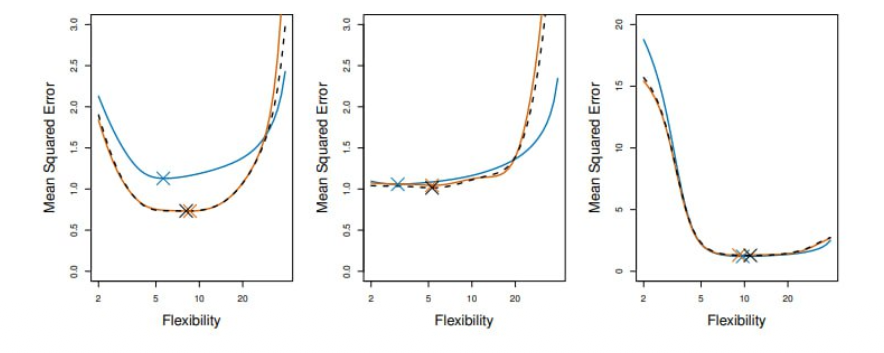
\includegraphics[width=\textwidth]{pictures/23-graphic.png}
  \end{center}
\end{frame}

%% K-Fold: цель + минимум
\begin{frame}
  \frametitle{K-блочная кросс-валидация: цель}

  Основная цель кросс-валидации~--- определить, насколько хорошо выбранная статистическая модель будет работать на независимых данных.

  \vspace{0.3cm}

  Нас интересует прежде всего \textbf{положение минимума} на кривой оценки тестовой MSE, а не само точное значение ошибки. Это связано с тем, что кросс-валидацию часто применяют для сравнения нескольких моделей или для выбора уровня гибкости одной модели, чтобы найти вариант с наименьшей тестовой ошибкой.

\end{frame}

%% K-Fold: bias-variance (слайды 25-27)
\begin{frame}
  \frametitle{K-блочная кросс-валидация: компромисс смещение--дисперсия}

  Помимо вычислительного преимущества перед LOOCV, k-блочная кросс-валидация зачастую даёт \textbf{более точные} оценки тестовой ошибки. Причина кроется в компромиссе между смещением и дисперсией.

\end{frame}

\begin{frame}
  \frametitle{K-блочная кросс-валидация: компромисс смещение--дисперсия}

  Помимо вычислительного преимущества перед LOOCV, k-блочная кросс-валидация зачастую даёт \textbf{более точные} оценки тестовой ошибки.

  \vspace{0.3cm}

  K-блочная кросс-валидация занимает промежуточное положение по смещению: оно выше, чем у LOOCV, но ниже, чем у валидации отложенной выборкой.

\end{frame}

\begin{frame}
  \frametitle{K-блочная кросс-валидация: компромисс смещение--дисперсия}

  Помимо вычислительного преимущества перед LOOCV, k-блочная кросс-валидация зачастую даёт \textbf{более точные} оценки тестовой ошибки.

  \vspace{0.2cm}

  K-блочная CV занимает промежуточное положение по смещению: оно выше, чем у LOOCV, но ниже, чем у валидации отложенной выборкой.

  \vspace{0.2cm}

  Однако необходимо учитывать и дисперсию процедуры. У LOOCV дисперсия \textbf{выше}, чем у k-блочной CV. При LOOCV мы усредняем результаты $n$ моделей, каждая из которых обучена на почти идентичном множестве данных; следовательно, эти результаты \textbf{сильно коррелированы}. Среднее большого числа сильно коррелированных величин обладает более высокой дисперсией.

\end{frame}

%% ============================================================
%% BOOTSTRAP (слайды 28-39)
%% ============================================================

\begin{frame}
  \frametitle{Бутстрэп}

  Бутстрэп~--- это мощный инструмент для количественной оценки неопределённости заданной статистической оценки или метода машинного обучения.

\end{frame}

\begin{frame}
  \frametitle{Бутстрэп}

  Бутстрэп~--- это мощный инструмент для количественной оценки неопределённости заданной статистической оценки или метода машинного обучения.

  \vspace{0.3cm}

  Предположим, мы хотим вложить фиксированную сумму в два финансовых актива, доходности которых~--- случайные величины $X$ и $Y$. Долю $\alpha$ вкладываем в $X$, а оставшуюся часть $(1 - \alpha)$~--- в $Y$.

\end{frame}

\begin{frame}
  \frametitle{Бутстрэп}

  Бутстрэп~--- это мощный инструмент для количественной оценки неопределённости заданной статистической оценки или метода машинного обучения.

  \vspace{0.3cm}

  Предположим, мы хотим вложить фиксированную сумму в два финансовых актива, доходности которых~--- случайные величины $X$ и $Y$. Долю $\alpha$ вкладываем в $X$, а оставшуюся часть $(1 - \alpha)$~--- в $Y$.

  \vspace{0.3cm}

  Наша задача~--- подобрать $\alpha$ так, чтобы минимизировать суммарный риск, то есть дисперсию портфеля.

\end{frame}

%% Bootstrap: формулы alpha
\begin{frame}
  \frametitle{Бутстрэп: оптимальное $\alpha$}

  Другими словами, мы хотим минимизировать $\text{Var}(\alpha X + (1 - \alpha) Y)$

\end{frame}

\begin{frame}
  \frametitle{Бутстрэп: оптимальное $\alpha$}

  Другими словами, мы хотим минимизировать $\text{Var}(\alpha X + (1 - \alpha) Y)$

  $$\alpha = \frac{\sigma^2_Y - \sigma_{XY}}{\sigma^2_X + \sigma^2_Y - 2\sigma_{XY}}$$

\end{frame}

\begin{frame}
  \frametitle{Бутстрэп: оптимальное $\alpha$}

  Другими словами, мы хотим минимизировать $\text{Var}(\alpha X + (1 - \alpha) Y)$

  $$\alpha = \frac{\sigma^2_Y - \sigma_{XY}}{\sigma^2_X + \sigma^2_Y - 2\sigma_{XY}}$$

  На практике значения $\sigma^2_X$, $\sigma^2_Y$ и $\sigma_{XY}$ неизвестны. Мы можем вычислить их оценки: $\hat{\sigma}^2_X$, $\hat{\sigma}^2_Y$ и $\hat{\sigma}_{XY}$

\end{frame}

\begin{frame}
  \frametitle{Бутстрэп: оценка $\alpha$}

  Тогда оценка значения $\alpha$:

  $$\hat{\alpha} = \frac{\hat{\sigma}^2_Y - \hat{\sigma}_{XY}}{\hat{\sigma}^2_X + \hat{\sigma}^2_Y - 2\hat{\sigma}_{XY}}$$

\end{frame}

%% Bootstrap: моделирование
\begin{frame}
  \frametitle{Бутстрэп: оценивание $\alpha$ на симуляции}

  Для оценки $\alpha$ мы можем смоделировать 100 пар доходностей инвестиций $X$ и $Y$. По ним вычисляются оценки $\sigma^2_X$, $\sigma^2_Y$ и $\sigma_{XY}$, а затем~--- оценка $\alpha$.

  \vspace{0.2cm}

  Естественно оценить стандартное отклонение $\hat{\alpha}$.

\end{frame}

\begin{frame}
  \frametitle{Бутстрэп: оценивание $\alpha$ на симуляции}

  Для оценки $\alpha$ смоделируем 100 пар доходностей $X$ и $Y$, вычислим оценку $\alpha$.

  Повторив процедуру 1000 раз, усредним результат.

  $$\bar{\alpha} = \frac{1}{1000} \sum_{r=1}^{1000} \hat{\alpha}_r = 0.5996$$

  При истинных характеристиках данных: $\sigma^2_X = 1$, $\sigma^2_Y = 1.25$, $\sigma_{XY} = 0.5$ и $\alpha = 0.6$

\end{frame}

%% Bootstrap: гистограммы
\begin{frame}
  \frametitle{Бутстрэп: распределение оценок}

  \begin{center}
  \begin{tikzpicture}[scale=0.55]
    \begin{axis}[
      width=6cm, height=5.5cm,
      xlabel={$\alpha$}, ylabel={Частота},
      xmin=0.35, xmax=0.95, ymin=0, ymax=250,
      grid=major, grid style={gray!15},
      title={\scriptsize Истинные выборки},
      ybar interval, fill=orange!60, draw=orange!80,
    ]
    \addplot coordinates {
      (0.38,15)(0.43,35)(0.48,70)(0.53,165)(0.58,235)(0.63,230)(0.68,130)(0.73,85)(0.78,25)(0.83,10)(0.88,0)
    };
    \draw[magenta, thick] (axis cs:0.6,0) -- (axis cs:0.6,250);
    \end{axis}
  \end{tikzpicture}
  \hspace{0.2cm}
  \begin{tikzpicture}[scale=0.55]
    \begin{axis}[
      width=6cm, height=5.5cm,
      xlabel={$\alpha$}, ylabel={Частота},
      xmin=0.25, xmax=0.95, ymin=0, ymax=250,
      grid=major, grid style={gray!15},
      title={\scriptsize Бутстрэп-выборки},
      ybar interval, fill=blue!50, draw=blue!70,
    ]
    \addplot coordinates {
      (0.28,10)(0.33,25)(0.38,50)(0.43,125)(0.48,200)(0.53,240)(0.58,210)(0.63,90)(0.68,35)(0.73,10)(0.78,5)(0.83,0)
    };
    \draw[magenta, thick] (axis cs:0.6,0) -- (axis cs:0.6,250);
    \end{axis}
  \end{tikzpicture}
  \end{center}

  \vspace{0.1cm}
  \begin{center}
  \small Розовая линия~--- истинное значение $\alpha = 0.6$
  \end{center}
\end{frame}

%% Bootstrap: идея
\begin{frame}
  \frametitle{Бутстрэп: основная идея}

  На практике мы не можем генерировать новые выборки из исходной генеральной совокупности. Однако метод бутстрэпа позволяет нам использовать компьютер для имитации процесса получения новых наборов данных, чтобы оценить вариабельность $\hat{\alpha}$ без дополнительных выборок.

  \vspace{0.3cm}

  Вместо многократного извлечения независимых наборов из генеральной совокупности мы формируем различные наборы путём \textbf{повторной выборки с возвращением} из имеющихся данных.

\end{frame}

%% Bootstrap: схема (TikZ)
\begin{frame}
  \frametitle{Бутстрэп: схема}
  \begin{center}
  \begin{tikzpicture}[
    scale=0.72,
    every node/.style={font=\scriptsize},
  ]
    % Исходные данные
    \node[draw, thick, minimum width=2.5cm, minimum height=2cm] (orig) at (0,0) {};
    \node[above] at (orig.north) {\small Исходные данные ($Z$)};
    \node at (0, 0.5) {Набл. 1: (4.3, 2.4)};
    \node at (0, 0) {Набл. 2: (2.1, 1.1)};
    \node at (0, -0.5) {Набл. 3: (5.3, 2.8)};

    % Z*1
    \node[draw, thick, minimum width=2.5cm, minimum height=2cm] (z1) at (6, 3) {};
    \node[above] at (z1.north) {$Z^{*1}$};
    \node at (6, 3.5) {3: (5.3, 2.8)};
    \node at (6, 3.0) {1: (4.3, 2.4)};
    \node at (6, 2.5) {3: (5.3, 2.8)};
    \draw[->, thick] (orig.east) -- (z1.west);
    \node at (9.5, 3) {$\longrightarrow \hat{\alpha}^{*1}$};

    % Z*2
    \node[draw, thick, minimum width=2.5cm, minimum height=2cm] (z2) at (6, 0) {};
    \node[above] at (z2.north) {$Z^{*2}$};
    \node at (6, 0.5) {2: (2.1, 1.1)};
    \node at (6, 0.0) {3: (5.3, 2.8)};
    \node at (6, -0.5) {1: (4.3, 2.4)};
    \draw[->, thick] (orig.east) -- (z2.west);
    \node at (9.5, 0) {$\longrightarrow \hat{\alpha}^{*2}$};

    % Точки
    \node at (6, -1.5) {$\vdots$};
    \node at (9.5, -1.5) {$\vdots$};

    % Z*B
    \node[draw, thick, minimum width=2.5cm, minimum height=2cm] (zb) at (6, -3.5) {};
    \node[above] at (zb.north) {$Z^{*B}$};
    \node at (6, -3.0) {2: (2.1, 1.1)};
    \node at (6, -3.5) {2: (2.1, 1.1)};
    \node at (6, -4.0) {1: (4.3, 2.4)};
    \draw[->, thick] (orig.east) -- (zb.west);
    \node at (9.5, -3.5) {$\longrightarrow \hat{\alpha}^{*B}$};
  \end{tikzpicture}
  \end{center}
\end{frame}

%% Bootstrap: процедура + формула SE
\begin{frame}
  \frametitle{Бутстрэп: процедура}

  Рассмотрим набор из $n = 3$ наблюдений. Из исходных данных случайным образом извлекаем $n$ наблюдений \textbf{с возвращением}, формируя бутстрэп-выборку $Z^{*1}$. Так как выборка производится с возвращением, одно и то же наблюдение может встретиться несколько раз.

  \vspace{0.3cm}

  По $Z^{*1}$ вычисляем новую оценку $\hat{\alpha}^{*1}$. Процедура повторяется $B$ раз, что даёт $B$ различных бутстрэп-выборок $Z^{*1}, Z^{*2}, \ldots, Z^{*B}$ и $B$ соответствующих оценок $\hat{\alpha}^{*1}, \hat{\alpha}^{*2}, \ldots, \hat{\alpha}^{*B}$.

\end{frame}

\begin{frame}
  \frametitle{Бутстрэп: стандартная ошибка}

  По $B$ бутстрэп-оценкам $\hat{\alpha}^{*1}, \hat{\alpha}^{*2}, \ldots, \hat{\alpha}^{*B}$ можно вычислить стандартную ошибку:

  $$SE_B(\hat{\alpha}) = \sqrt{\frac{1}{B-1} \sum_{r=1}^{B} \left(\hat{\alpha}^{*r} - \frac{1}{B} \sum_{r'=1}^{B} \hat{\alpha}^{*r'}\right)^2}$$

\end{frame}

%% ============================================================
%% ИТОГИ (слайд 40)
%% ============================================================

\begin{frame}
  \frametitle{Итоги}

  \begin{itemize}
    \item \textbf{Валидация отложенной выборкой}: просто, но с высокой дисперсией оценки и неэффективным использованием данных
    \vspace{0.3cm}
    \item \textbf{LOOCV}: малое смещение, детерминированный результат, однако вычислительно затратный и может обладать высокой дисперсией
    \vspace{0.3cm}
    \item \textbf{K-блочная кросс-валидация}: практичный компромисс между смещением и дисперсией; обычно используют $k = 5$ или $k = 10$
    \vspace{0.3cm}
    \item \textbf{Бутстрэп}: универсальный инструмент для оценки неопределённости через повторную выборку с возвращением
  \end{itemize}
\end{frame}

\end{document}
